\usection{Procedimiento Metodológico}

\usubsection{Análisis del sistema de monitoreo acústico para generar alertas en casos de emergencia}

La definición de la metodología y los requerimientos del sistema se basó en un análisis de literatura existente, estudios previos, noticias de incidentes y la identificación de sus potenciales usuarios. Se determinó que el sistema está dirigido a cualquier individuo que, por un evento súbito como una caída o una agresión, se encuentre en una situación de vulnerabilidad que le impida solicitar ayuda. El análisis se enfocó en perfiles prioritarios con mayor exposición a estos riesgos, como adultos mayores que viven solos, personas con condiciones médicas que limitan su movilidad y potenciales víctimas de robos o violencia doméstica. La característica común de estos grupos es la posible incapacidad de interactuar con un dispositivo durante la emergencia, lo cual estableció el funcionamiento autónomo y pasivo como un requisito técnico clave. El sistema debe, por tanto, detectar la anomalía e iniciar una alerta sin depender de la acción del usuario, justificando así la elección de un monitoreo acústico continuo. Este requisito define el desafío técnico central el cómo lograr que el sistema interprete el entorno sonoro de manera inteligente. Para abordar dicho desafío, se realizó una revisión de artículos científicos y casos de estudio sobre el análisis de audio y la detección de anomalías. La investigación comenzó explorando la interpretación del audio crudo, donde se identificó que el uso de modelos de clasificación pre-entrenados, como la arquitectura YAMNet, era el punto de partida más efectivo para convertir el sonido ambiental en una secuencia de eventos etiquetados. Una vez resuelto ``el qué'' (la clasificación), el análisis se centró en cuándo un patrón es ``anómalo''. Se evaluaron diferentes enfoques para analizar dicha secuencia, desde cadenas de Markov para cambios de estado simples hasta métodos no supervisados como Isolation Forest y arquitecturas de aprendizaje profundo como las redes LSTM. Este recorrido llevó a la conclusión de que la estrategia más robusta era descomponer el problema, primero usar un clasificador de alto nivel para traducir el sonido y segundo, aplicar modelos de detección de anomalías sobre esa secuencia de datos estructurados para analizar el comportamiento.

\usubsubsection{Revisión de estudios previos y fundamentos teóricos}

Se revisaron diversos estudios previos sobre el procesamiento de señales de audio y la clasificación de eventos sonoros anómalos. Entre ellos, destacan los trabajos de \citeauthor{malmberg_real-time_2021} \citeyear{malmberg_real-time_2021}, quienes abordaron la implementación de modelos de aprendizaje automático en dispositivos edge para la clasificación de audio en tiempo real. Su investigación se centró en el uso del modelo YAMNet, reentrenado para detectar eventos acústicos como disparos, rotura de cristales y habla humana. Este estudio demostró que, aunque existe una ligera pérdida de precisión al utilizar versiones optimizadas como TensorFlow Lite, los resultados son comparables a los de la versión completa, lo que abre la posibilidad de trabajar con dispositivos de bajo consumo y recursos limitados, como la Raspberry Pi o el ESP32 \cite{malmberg_real-time_2021}.

El método para detectar la actividad general en el entorno se inspiró en el trabajo de \citeauthor{torija_metodologia_2018} \citeyear{torija_metodologia_2018}. Su investigación, aunque centrada en ambientes urbanos, proporcionó un marco de referencia para analizar los niveles de energía sonora, demostrando que los cambios bruscos en dichos niveles son indicadores fiables de eventos críticos. Este proyecto extiende ese principio para un análisis dual: no solo se utiliza para detectar ``picos de actividad'' (un incremento brusco de energía que puede sugerir un grito o un golpe), sino también para su opuesto, la ``ausencia de actividad''. Un período de silencio prolongado e inusual, que representa una caída significativa por debajo del nivel de energía normal, es igualmente un potente indicador de una posible anomalía. Este doble enfoque se fundamenta en la premisa demostrada por \citeauthor{torija_metodologia_2018} \citeyear{torija_metodologia_2018}, quienes establecieron que un análisis centrado en los niveles de energía sonora es un método eficaz para diferenciar el ruido de fondo de eventos acústicos críticos.

En cuanto a los fundamentos teóricos, el sistema se apoya en principios de la inteligencia artificial, campo que, según \citeauthor{russell_artificial_2022} \citeyear{russell_artificial_2022}, se enfoca en el desarrollo de sistemas capaces de percibir y actuar sobre su entorno. En este proyecto, dicha capacidad de percepción se logra mediante una combinación de modelos de aprendizaje profundo (deep learning). Para la clasificación inicial de los sonidos, se emplean arquitecturas como las redes neuronales convolucionales (CNN). Posteriormente, para el análisis de la secuencia de eventos y la detección de anomalías, se integra una combinación de modelos no supervisados como Isolation Forest y redes neuronales recurrentes (LSTM). Esta arquitectura de software, que utiliza distintos componentes de IA para sus tareas de percepción y análisis, se fundamenta en los conceptos teóricos establecidos por autores de referencia en el campo (Russell y Norvig, 2022).

\usubsubsection{Selección de hardware y dispositivos Edge}
% Todo: Revisar esto despues
Para la implementación del sistema, se realizó una evaluación de hardware con un enfoque en dispositivos de Edge Computing. La elección se centró en plataformas capaces de procesar datos localmente para reducir la latencia y la dependencia de la nube, como lo describen \citeauthor{shi_edge_2016} \citeyear{shi_edge_2016}. En este contexto, se seleccionó la Raspberry Pi como la plataforma de desarrollo, dada su versatilidad para integrar componentes como micrófonos y su amplia conectividad, características que la hacen ideal para aplicaciones de IoT y análisis en tiempo real según \citeauthor{richardson_getting_2016} \citeyear{richardson_getting_2016}. (incluir que para que el sistema sea consciente de las rutinas del entorno (y es del entorno y no de la persona xq siempre estan fijos en el mismo lugar) debe correr modelos con los datos generandos en ese entorno especifico, lo que  implicaria un gran servidor muy costoso con multiples modelos corriendo por entorno o un dispositivo edge que corra los modelos localmente y aprenda del entorno especifico)

\usubsubsection{Limitaciones y desafíos técnicos}

Durante el análisis inicial, se identificaron varias limitaciones y desafíos técnicos que podrían afectar el desempeño del sistema. Entre ellos, destacan:

\begin{enumerate}
      \item Limitaciones tecnológicas: El rendimiento del sistema está directamente condicionado por tres factores: la calidad del sensor acústico para una captura de audio fiel, la capacidad de procesamiento del hardware de borde para ejecutar los modelos sin latencia, y la presencia de ruido ambiental, que puede enmascarar o ser confundido con eventos anómalos.
      \item Limitaciones de datos: La recolección de suficientes muestras de sonidos para entrenar el modelo puede ser limitada, lo que puede comprometer el funcionamiento del sistema en escenarios no previstos. Para abordar este desafío, se consideró la posibilidad de utilizar datasets públicos y el uso de modelos preentrenados.
      \item Privacidad y seguridad: El desafío ético y técnico de monitorear un entorno privado. Se abordó estableciendo como requisito fundamental el procesamiento 100\% local (Edge AI), sin almacenar ni transmitir grabaciones de audio, para garantizar la confidencialidad del usuario.
\end{enumerate}

\usubsubsection{Requerimientos Funcionales}

\begin{enumerate}
      \item El sistema debe capturar el audio ambiental de forma continua a través de los micrófonos designados.
      \item El sistema debe procesar el audio capturado para clasificarlo en eventos sonoros predefinidos (ej. voz, silencio, golpe, etc.) utilizando sus modelos de IA.
      \item El sistema debe aprender y mantener un perfil de la actividad acústica ``normal'' del entorno, basado en la secuencia y horario de los sonidos clasificados.
      \item El sistema debe comparar la actividad en tiempo real con el perfil de normalidad para detectar patrones anómalos.
      \item El sistema debe realizar una consulta verbal al usuario (ej. ``¿Está todo bien?'') cuando se detecte una anomalía.
      \item Permitir al usuario responder que está bien en caso de que haya un falso positivo o se presente una posible situación de emergencia.
      \item El sistema debe enviar notificaciones de emergencia a una lista de contactos predefinidos si una anomalía es crítica o si no se recibe respuesta a la consulta de verificación.
\end{enumerate}

\usubsubsection{Requerimientos no funcionales}

\begin{enumerate}
      \item Garantizar la seguridad y privacidad de los datos al no almacenar grabaciones de audio ni datos personales sensibles.
      \item Ser escalable para adaptarse a diferentes entornos y necesidades, permitiendo la integración de nuevos micrófonos o dispositivos de procesamiento según sea necesario.
      \item Mantener una alta disponibilidad para estar operativo las 24 horas del día, los 7 días de la semana, garantizando la detección continua de eventos sonoros críticos.
      \item Mejorar el uso de recursos de hardware, como la memoria y el procesamiento, para funcionar en dispositivos de bajo consumo, como la Raspberry Pi.
      \item Contar con una interfaz de usuario intuitiva que sea fácil de usar tanto para usuarios técnicos como no técnicos.
      \item Ser robusto y confiable para funcionar en entornos ruidosos y bajo condiciones variables, manteniendo una alta precisión en la detección de eventos sonoros.
      \item Facilitar el mantenimiento y actualización mediante un diseño modular que permita actualizaciones de software y hardware sin interrumpir su funcionamiento.
\end{enumerate}

\usubsubsection{Selección de Tecnologías}

Una vez definidos los requerimientos, se procedió a la selección de las tecnologías para cada capa del sistema. La elección se basó en criterios como el rendimiento en entornos de borde (Edge), la disponibilidad de código abierto, el costo y la compatibilidad entre componentes.

\uparagraph{Captura de Audio (Hardware)}

\begin{enumerate}
      \item \textbf{Micrófonos:} Para garantizar una captura de audio clara, se seleccionaron micrófonos con alta sensibilidad. Como señalan \citeauthor{torija_metodologia_2018} \citeyear{torija_metodologia_2018}, la calidad del sensor acústico es un factor determinante para la precisión en la detección de eventos.
      \item \textbf{Plataforma de Procesamiento (Raspberry Pi):} Se eligió la Raspberry Pi como el dispositivo de borde principal debido a su bajo costo, su comunidad de soporte y su capacidad para ejecutar los modelos de IA. Su versatilidad y opciones de conectividad la hacen ideal para prototipar proyectos de IoT y análisis en tiempo real \cite{richardson_getting_2016}.
\end{enumerate}

\uparagraph{Procesamiento y Lógica de Detección (Software)}

\begin{enumerate}
      \item Framework de IA (TensorFlow Lite): Para la ejecución de los modelos en el dispositivo, se optó por TensorFlow Lite. Esta es una versión optimizada de TensorFlow diseñada específicamente para hardware con recursos limitados, permitiendo una inferencia rápida y eficiente (Goldsborough, 2016).
      \item Modelo de Clasificación de Sonido (YAMNet): Se seleccionó YAMNet como el clasificador de audio base. Al ser un modelo pre-entrenado por Google en un dataset masivo (AudioSet), proporciona una base robusta para identificar una amplia gama de eventos acústicos generales sin necesidad de un entrenamiento desde cero.
      \item Modelos de Detección de Anomalías (Isolation Forest y LSTM): Para el análisis del comportamiento, se eligió una combinación de Isolation Forest, por su alta eficiencia para detectar anomalías puntuales, y un Autoencoder LSTM, por su capacidad para identificar patrones anómalos en secuencias temporales.
      \item Modelo de Detección de Palabras Clave (Vosk): Para la funcionalidad de activación por voz, se seleccionó la librería Vosk, un toolkit de reconocimiento de voz de código abierto que puede operar completamente offline en la Raspberry Pi, garantizando la privacidad
\end{enumerate}

\uparagraph{Capa de Notificación (Backend)}
\begin{enumerate}
      \item Framework del Servidor (NestJS): Para el sistema de envío de notificaciones, se seleccionó NestJS. Al ser un framework de Node.js escalable y basado en TypeScript, facilita la creación de un backend mantenible y eficiente, capaz de gestionar las alertas de forma segura \cite{sabo_nestjs_2020}.
\end{enumerate}

\usubsection{Diseño del sistema de monitoreo acústico para generar alertas en casos de emergencia}

\usubsubsection{Diseño de la arquitectura del sistema}

La arquitectura implementada se fundamenta en el modelo en capas, donde cada nivel cumple funciones específicas: captura de datos, clasificación de audio, detección de anomalías, gestión de eventos y almacenamiento. Estas capas no se ejecutan como módulos monolíticos, sino como procesos independientes que se comunican mediante un esquema pub/sub interno con Redis, lo que introduce un componente distribuido dentro del propio dispositivo. Según \citeauthor{tanenbaum2007distributed} \citeyear{tanenbaum2007distributed}, este tipo de combinaciones puede entenderse como una arquitectura híbrida, al integrar un estilo cliente-servidor con mecanismos de colaboración descentralizados. Además, el uso de un Raspberry Pi como nodo principal aproxima la solución al concepto de servidores al borde, en los cuales el procesamiento ocurre cerca de la fuente de datos para optimizar tiempos de respuesta y reducir la transmisión de información irrelevante. De esta manera, la propuesta logra unir la claridad del enfoque en capas con la flexibilidad de un sistema distribuido basado en microservicios locales.

\begin{enumerate}
      \item Capa de captación de audio: Esta capa corresponde al nivel más cercano al hardware y tiene como función principal la adquisición de datos acústicos mediante los micrófonos conectados al dispositivo Raspberry Pi. Se encarga de gestionar la interacción con el sistema operativo para acceder a las señales de audio en tiempo real y ponerlas a disposición del sistema a través de canales de comunicación internos. Su objetivo es abstraer la complejidad del hardware y garantizar que los datos se entreguen de forma continua a las capas superiores.
      \item Capa de clasificación de audio: Se encarga de analizar las señales acústicas para identificar patrones relevantes. En este nivel, múltiples agentes especializados procesan el flujo de audio con el fin de determinar la presencia de actividad, reconocer palabras clave y clasificar eventos característicos (como golpes, vidrios rotos o gritos). Los resultados de este procesamiento se estructuran en mensajes que representan descripciones semánticas de la señal, reduciendo el volumen de datos y facilitando la interpretación en etapas posteriores.
      \item Capa de detección de anomalías: En esta capa se aplican modelos de aprendizaje automático previamente entrenados (como Isolation Forest y LSTM) para diferenciar entre eventos normales y anormales. El sistema utiliza los datos clasificados por la capa anterior como entrada, evaluando si el comportamiento acústico observado corresponde a patrones esperados dentro del entorno o si, por el contrario, representa una desviación significativa. Esta capa constituye el núcleo analítico del sistema, ya que transforma datos objetivos en juicios de normalidad o anomalía.
      \item Capa de gestión de alertas: La función de esta capa es decidir cuáles de las anomalías detectadas deben escalarse como alertas reales. Para ello, aplica un conjunto de reglas predefinidas que consideran factores contextuales, como los horarios (por ejemplo, diferenciar entre actividad normal en horas diurnas y actividad sospechosa durante la madrugada) o la naturaleza del evento (gritos de auxilio, sonidos de ruptura). Además, esta capa gestiona la interacción con el usuario mediante consultas verbales para validar la situación antes de enviar notificaciones externas. Su propósito es minimizar los falsos positivos y asegurar que solo las situaciones críticas generen una respuesta.
      \item Capa de gestión de datos: Esta capa centraliza la persistencia y organización de la información recolectada y procesada por el sistema. Su propósito es almacenar los registros de eventos, tanto normales como anómalos, en estructuras que permitan su posterior análisis. Asimismo, prepara los conjuntos de datos necesarios para el reentrenamiento de los modelos de detección de anomalías, asegurando que el sistema pueda mejorar progresivamente su desempeño y adaptarse a nuevas condiciones acústicas en el entorno.
      \item Capa de notificaciones: Tiene como responsabilidad la comunicación con el usuario final o con sistemas externos de monitoreo. Actualmente, este módulo envía alertas validadas a través de servicios de mensajería como Telegram y protocolos de correo electrónico (SMTP). Su diseño es extensible, lo que permite incorporar otros canales de comunicación en el futuro. La existencia de esta capa garantiza que la información crítica llegue de forma oportuna a los responsables de la toma de decisiones.
      
      \begin{figure}[ht!]
            \centering
            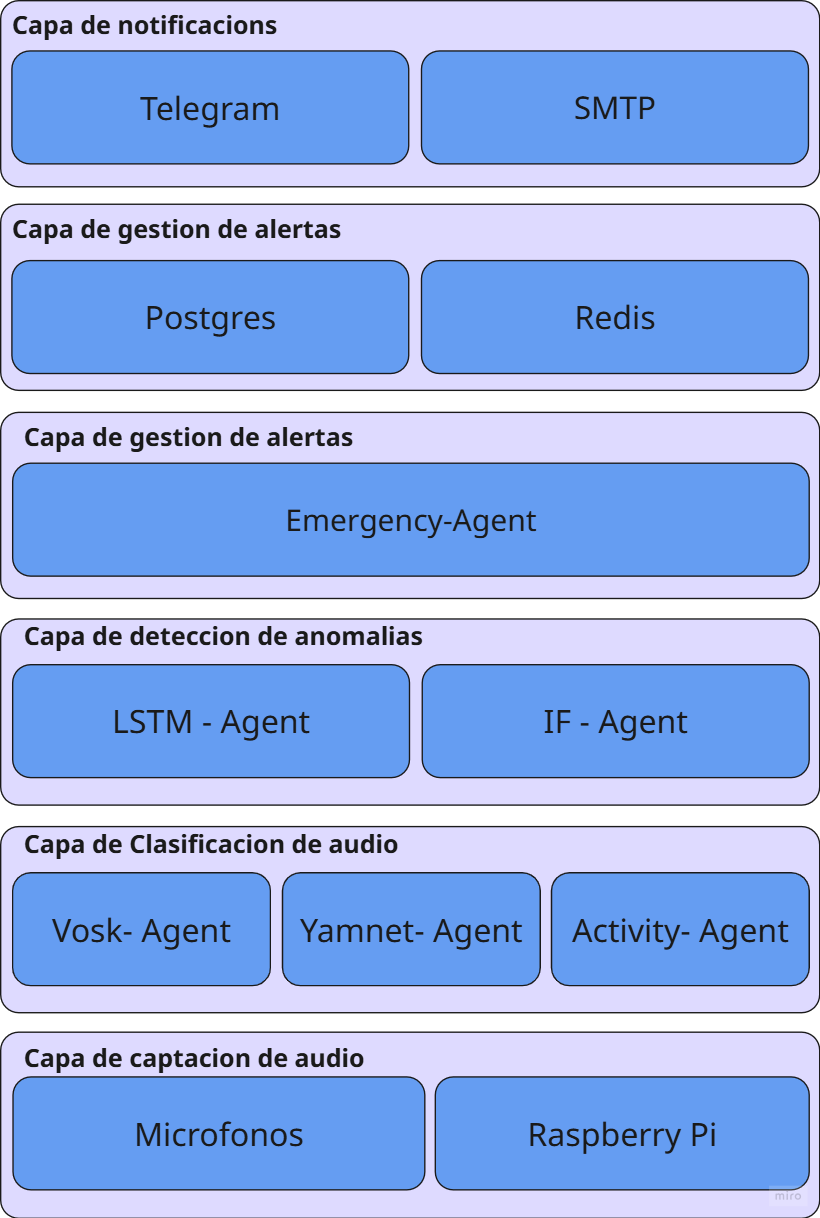
\includegraphics[width=0.40\textwidth]{Arquitectura/Arquitectura.png}
            \caption{Arquitectura del sistema de monitoreo acústico para generar alertas en casos de emergencia}
            \label{fig:arquitectura}
      \end{figure}
\end{enumerate}

\usubsubsection{Diseño de la Inteligencia Artificial}

En esta etapa, se diseñó un sistema de inteligencia artificial que combina modelos avanzados para el análisis de audio. El sistema utiliza YAMNet, un modelo pre-entrenado por Google, para la clasificación precisa de eventos sonoros. Para la detección no supervisada de anomalías en secuencias acústicas, integra autoencoders con LSTM, capaces de aprender patrones temporales, y Isolation Forest, un algoritmo de detección de anomalías. A continuación, se describen en detalle cada uno de estos componentes, su funcionamiento y cómo se integraron en el sistema.

\uparagraph{Yamnet}

El modelo YAMNet fue seleccionado como la base para la clasificación de eventos sonoros debido a su capacidad comprobada en tareas de reconocimiento de audio y su eficiencia en dispositivos con recursos limitados. Desarrollado por Google, YAMNet es un modelo preentrenado disponible en formato TFLite, lo que lo hace ideal para su implementación en sistemas embebidos o de bajo consumo computacional. Este modelo fue descargado desde la plataforma Kaggle, en su página oficial. YAMNet está entrenado sobre el conjunto de datos AudioSet, que contiene más de 2 millones de segmentos de audio etiquetados con 521 clases de eventos sonoros, como gritos, ladridos, música, ruidos ambientales, entre otros. Esta amplia cobertura de clases lo convierte en una herramienta versátil para la detección de eventos críticos.

La arquitectura de YAMNet se basa en MobileNet v1, una red neuronal convolucional (CNN) diseñada específicamente para aplicaciones móviles y embebidas. Esta arquitectura permite ejecutar el modelo en dispositivos con limitaciones de hardware sin sacrificar el rendimiento. El modelo acepta como entrada una forma de onda de audio en formato mono, muestreada a 16 kHz, y normalizada en el rango de [-1.0, +1.0]. Internamente, YAMNet divide la forma de onda en ventanas de 0.96 segundos con un salto (hop) de 0.48 segundos, lo que permite analizar el audio en tiempo real. Cada ventana se procesa de manera independiente, generando tres tipos de salidas: scores, que contienen las puntuaciones de predicción para cada una de las 521 clases; embeddings, que representan características de alto nivel extraídas del audio.

Para adaptar YAMNet a la tarea específica de detección de eventos críticos, como gritos, caídas y rotura de cristales, se utilizó la salida de embeddings como entrada para un clasificador adicional. Este enfoque, conocido como transfer learning, permite aprovechar el conocimiento preentrenado de YAMNet y ajustarlo a las necesidades del sistema sin requerir un entrenamiento extensivo desde cero.

\uparagraph{LSTM}

Las redes neuronales recurrentes (RNN) fueron diseñadas para procesar datos secuenciales, pero se enfrentaban a un desafío importante: la incapacidad de retener información a largo plazo debido al problema del desvanecimiento del gradiente \cite{heaton2018ian}. Para superar esta limitación crítica, \citeauthor{hochreiter1997long} \citeyear{hochreiter1997long} desarrollaron las redes LSTM. Esta arquitectura innovadora no solo procesa secuencias de manera efectiva, sino que también introduce un mecanismo de memoria que le permite recordar información relevante por largos periodos, lo que era un obstáculo insalvable para las RNN tradicionales.

La capacidad distintiva de una red LSTM radica en su celda de memoria (cell state), que actúa como una cinta transportadora que lleva información relevante a lo largo de toda la secuencia de la red. A diferencia de una neurona simple, una celda LSTM está equipada con tres ``puertas'' reguladoras: la puerta de olvido (forget gate), la de entrada (input gate) y la de salida (output gate). Estas puertas, controladas por funciones sigmoides, deciden qué información debe ser eliminada, qué información nueva debe ser agregada y qué información debe ser utilizada para generar la salida, respectivamente \cite{heaton2018ian}.

La interacción entre estas puertas es lo que le da a las LSTM su poder. La puerta de olvido revisa el estado anterior y la entrada actual para determinar qué datos ya no son necesarios, limpiando la memoria. Luego, la puerta de entrada evalúa la nueva información y decide si es lo suficientemente importante para ser almacenada en la celda de memoria. Finalmente, la puerta de salida toma decisiones sobre la información contenida en la celda de memoria y la entrada actual para generar el valor de salida de la célula, permitiendo que la red utilice el conocimiento aprendido para una tarea específica \cite{heaton2018ian}.

Gracias a este de control de memoria, las LSTM han demostrado ser efectivas en una amplia gama de aplicaciones. En el procesamiento del lenguaje natural (NLP), son fundamentales para la traducción automática y la generación de texto, ya que pueden capturar las dependencias gramaticales a largo plazo. También son cruciales en la detección de anomalías en secuencias de datos, como el audio, donde pueden aprender los patrones de sonido normales para luego identificar desviaciones que indican la presencia de una anomalía. Su éxito se debe a que superan la limitación de las RNN, permitiendo un mejor manejo de las dependencias a largo plazo \cite{hochreiter1997long}.

\uparagraph{Isolation Forest (Bosque de Aislamiento)}

A diferencia de la mayoría de los algoritmos de detección de anomalías, que intentan construir un perfil complejo de los datos ``normales'' para luego identificar lo que no encaja, Isolation Forest (IF) se basa en un principio mucho más directo y eficiente. La premisa fundamental es que las anomalías son, por definición, ``pocas y diferentes'', lo que las hace más susceptibles a ser aisladas que los puntos de datos normales \cite{liu2012isolation}.

El algoritmo funciona construyendo un conjunto de árboles de decisión aleatorios, conocidos como ``árboles de aislamiento'' (isolation trees). Para cada árbol, el conjunto de datos se particiona recursivamente seleccionando un atributo al azar y luego un valor de división aleatorio entre el valor máximo y mínimo de ese atributo. Este proceso de división aleatoria se repite hasta que cada punto de datos queda aislado en un nodo hoja del árbol. La idea central es que los puntos anómalos, al ser diferentes y estar más alejados de las concentraciones de datos normales, requerirán menos particiones para ser aislados \cite{liu2012isolation}.

La ``anomalía'' de un punto se mide calculando la longitud del camino (path length) desde la raíz del árbol hasta el nodo hoja que lo contiene. Los puntos normales, que se encuentran en regiones densas, necesitarán muchos más cortes para ser aislados, resultando en caminos más largos. En contraste, las anomalías, que se encuentran en zonas de baja densidad, serán aisladas con muy pocos cortes, resultando en caminos muy cortos. El puntaje final de anomalía para cada punto se calcula promediando la longitud de su camino a través de todos los árboles del bosque, lo que hace que el resultado sea robusto y fiable \cite{liu2012isolation}.

Gracias a su simplicidad y a no depender de cálculos de distancia o densidad, Isolation Forest es extremadamente rápido y tiene un bajo consumo de memoria. Estas características lo convierten en un candidato ideal para la detección de anomalías en tiempo real sobre grandes volúmenes de datos, y es particularmente adecuado para ser implementado en dispositivos de borde (Edge) con recursos computacionales limitados, como es el caso de este proyecto.

\usubsection{Implementación del sistema de monitoreo acústico para generar alertas en casos de emergencia}

\usubsubsection{Iteraciones}

\begin{enumerate}
      \item Prototipo basado en esp32 y detección de intensidad de sonido

            \begin{figure}[ht!]
                  \centering
                  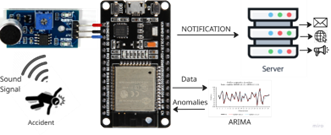
\includegraphics[width=0.65\textwidth]{Arquitectura/I1.png}
                  \caption{Prototipo basado en ESP32 y detección de intensidad de sonido}
                  \label{fig:prototipo1}
            \end{figure}

            Para el primer ciclo de desarrollo, y siguiendo una recomendación del tutor del proyecto, el objetivo fue validar la hipótesis de que se podían detectar anomalías a través del error de pronóstico de un modelo de series temporales. La estrategia consistía en utilizar un modelo estadístico como ARIMA para predecir el comportamiento sonoro ``normal'', de modo que cualquier diferencia significativa entre el valor predicho y el valor real observado fuera clasificada como una anomalía. El diseño del prototipo para probar este enfoque se inspiró en metodologías documentadas para sistemas IoT \cite{luis2024desarrollo} y consistió en un dispositivo de captura basado en un microcontrolador ESP32, que transmitía el audio a un servidor local (Raspberry Pi 4) para su análisis con el modelo ARIMA.

            Sin embargo, durante la fase de evaluación, este enfoque demostró ser fundamentalmente inviable. El problema de fondo no fue solo que el modelo ARIMA tuviera limitaciones, sino que su propio proceso de parametrización resultó ser incompatible con la naturaleza del problema de investigación.

            La parametrización de ARIMA busca encontrar una ``receta'' estadística fija (los valores p,d,q) que describa la estructura de la serie de tiempo. Este enfoque funciona bien cuando el proceso que genera los datos es estable y predecible. No obstante, el entorno acústico de un hogar es todo lo contrario, lo que reveló las siguientes incompatibilidades críticas:

            \begin{itemize}
                  \item Naturaleza Dinámica y No Estacionaria: La principal barrera fue que las señales acústicas de un ambiente domestico son altamente no estacionarias. Parametrizar ARIMA es como tomar una foto de las reglas estadísticas del sonido en un momento dado, pero el sonido de un hogar es una ``película'' que cambia constantemente. La ``receta'' estadística que describe los sonidos de una mañana activa (conversaciones, desayuno) es completamente diferente a la de una tarde silenciosa o una noche con la televisión encendida. Un modelo con parámetros fijos, por definición, no puede adaptarse a estos cambios de contexto, lo cual viola el supuesto fundamental de estacionariedad que ARIMA necesita para operar de forma fiable.
                  \item Complejidad y No Linealidad: El proceso de parametrización de ARIMA asume que las relaciones en los datos son, en su mayoría, lineales. Sin embargo, los eventos sonoros de una emergencia (un grito, un golpe fuerte, un cristal rompiéndose) son eventos abruptos y no lineales. Un modelo lineal es incapaz de capturar la complejidad de estas interacciones, lo que limita severamente su capacidad para detectar las anomalías más críticas.
                  \item Carencia de Contexto Externo: La ``receta'' (p,d,q) de ARIMA solo se basa en los valores pasados de la propia señal de audio. El modelo es ``ciego'' a información contextual crucial, como la hora del día, el día de la semana o si hay personas en casa. Un sonido, como pasos rápidos, puede ser normal a las 3 PM, pero una anomalía crítica a las 3 AM. Al no poder incorporar variables externas, ARIMA es incapaz de realizar esta distinción.
                  \item Baja Adaptabilidad a Cambios Súbitos: Como consecuencia de su parametrización fija, ARIMA asume que el comportamiento pasado se mantendrá en el futuro. Esto lo hace poco adaptable a rupturas estructurales en el entorno, como el inicio de una reunión social o una tormenta, respondiendo pobremente ante eventos atípicos.
            \end{itemize}

            Estas limitaciones nos llevaron a considerar enfoques más flexibles y robustos, capaces de adaptarse a la dinámica cambiante del entorno doméstico y a las características complejas de las señales de audio.

      \item Esp32 con micrófonos de señales de audio (Inmp441 Omnidireccional) y prophet

            \begin{figure}[ht!]
                  \centering
                  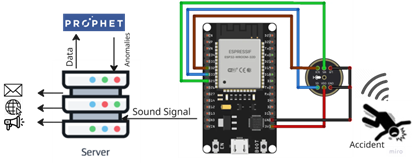
\includegraphics[width=0.85\textwidth]{Arquitectura/I2.png}
                  \caption{Diseño de prototipo de esp32 con micrófono de señales de audio y prophet}
                  \label{fig:prototipo2}
            \end{figure}

            En una segunda iteración, se abandonó la rigidez del modelo ARIMA en favor de un enfoque más flexible. Aunque se mantuvo la arquitectura de hardware basada en el microcontrolador ESP32, se integraron micrófonos omnidireccionales INMP441 para garantizar una captura de señales acústicas de alta fidelidad. A nivel de software, se reemplazó el modelo ARIMA por Prophet, una librería de pronóstico de series temporales desarrollada por Facebook, diseñada específicamente para superar las limitaciones del enfoque anterior.

            El modelo Prophet logró ajustarse a las variaciones periódicas del sonido ambiental, como los patrones de ruido diurnos y nocturnos. Sin embargo, durante las pruebas se identificó una limitación crítica: su mecanismo para suavizar datos e identificar tendencias a largo plazo provocaba que se descartaran los eventos de interés. Sonidos de corta duración y alta amplitud, como un golpe, un grito o la rotura de un cristal, eran filtrados por el modelo y no generaban ninguna alerta, ya que no formaban parte de un patrón estacional o de una tendencia.

            Esta observación llevó a la conclusión de que el enfoque de pronóstico de series temporales, independientemente del modelo utilizado, no era el adecuado para el objetivo del proyecto. El problema no era predecir la evolución del nivel de ruido, sino detectar eventos instantáneos y atípicos en el contenido de la señal acústica. Por lo tanto, se redefinió el problema como uno de detección de anomalías en tiempo real, lo que exigió un cambio completo en la estrategia de software.

            Para implementar esta nueva estrategia de detección de anomalías, se propuso un enfoque basado en una arquitectura de redes neuronales. La hipótesis de trabajo es que un modelo de este tipo puede aprender a caracterizar el perfil acústico ``normal'' de un entorno a partir de la extracción de características espectrales del audio. De esta forma, el sistema podría operar en tiempo real identificando cualquier desviación significativa de esa línea base aprendida y marcarla como una posible anomalía.

      \item Desarrollo de con dataset propio y modelo personalizado

            Inicialmente, la estrategia se centró en el desarrollo de un modelo de clasificación personalizado a partir de un conjunto de datos propio. El plan consistía en capturar y etiquetar una colección de sonidos de emergencia para entrenar una red neuronal diseñada específicamente para los escenarios de interés del proyecto.

            Sin embargo, a medida que avanzaba el desarrollo, la investigación sobre la robustez de los clasificadores acústicos reveló la verdadera magnitud del desafío. Se hizo evidente que para que un modelo pudiera generalizar y operar de manera fiable, necesitaría ser entrenado con un volumen de datos masivo. La literatura académica confirma que la efectividad de los modelos de aprendizaje profundo para audio depende directamente de la escala y diversidad de los datos, requiriendo a menudo millones de ejemplos para capturar la enorme variabilidad de los sonidos del mundo real \cite{gemmeke2017audio}. La tarea de construir un dataset de esa magnitud era logísticamente inviable para el proyecto.

            Fue precisamente durante esta etapa de investigación que se identificó YAMNet, una arquitectura de clasificación acústica ya pre-entrenada por Google. Este modelo fue entrenado sobre el corpus AudioSet, un extenso conjunto de datos que, como describen \citeauthor{gemmeke2017audio} \citeyear{gemmeke2017audio}, contiene más de dos millones de clips de audio de 10 segundos etiquetados a partir de una ontología de 527 clases de eventos sonoros. El descubrimiento de YAMNet ofrecía una solución directa al problema de la adquisición de datos a gran escala que se había identificado como el principal obstáculo.

            Ante esta situación, continuar con el desarrollo de un modelo propio habría significado un esfuerzo redundante. Por lo tanto, se tomó la decisión estratégica de descartar el enfoque personalizado y pivotar hacia la integración de YAMNet. Esta medida es una aplicación del paradigma de aprendizaje por transferencia (transfer learning), que permite aprovechar el conocimiento de un modelo ya entrenado en un gran dataset para resolver un problema específico con mayor eficiencia y fiabilidad, tal como analizan \citeauthor{pons2019deep} \citeyear{pons2019deep} en su trabajo sobre el impacto del tamaño del dataset en audio. Esto permitió enfocar los recursos del proyecto en la implementación del sistema final sobre una base tecnológica ya validada.

      \item Raspberry Pi, Yamnet, Cadenas de Markov

            \begin{figure}[ht!]
                  \centering
                  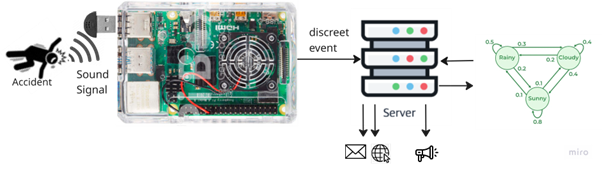
\includegraphics[width=0.85\textwidth]{Arquitectura/I4.png}
                  \caption{Prototipo con Raspberry Pi, Yamnet y Cadenas de Markov}
                  \label{fig:prototipo4}
            \end{figure}

            En esta cuarta iteración del prototipo, se migró la lógica de procesamiento desde el ESP32 hacia una Raspberry Pi, con mayor capacidad computacional, lo que permitió trabajar con señales de audio completas en lugar de limitarse a la intensidad. Se integraron micrófonos digitales de rango completo, capaces de capturar audio a frecuencias más altas y con mayor fidelidad, lo que permitió acceder a un contenido espectral más rico y útil para clasificación detallada.

            Con esta infraestructura, se incorporó YAMNet, un modelo de clasificación de audio en tiempo real basado en redes neuronales convolucionales entrenado con el dataset AudioSet de Google. YAMNet permite detectar y clasificar una gran variedad de eventos acústicos o (más de 500 categorías) como gritos, portazos, pasos, objetos cayendo, entre otros. Esta capacidad permitió dar un salto importante en la interpretación contextual del entorno sonoro.

            No obstante, Si bien YAMNet ofrecía una detección puntual efectiva de eventos sonoros, surgió la necesidad de dotar a dichos eventos de un significado secuencial y contextual. Para atender esta limitación, se optó por integrar un módulo de modelado probabilístico basado en cadenas de Márkov, con el fin de analizar la secuencia temporal de eventos y determinar si un patrón resultaba coherente con el comportamiento normal del entorno o, por el contrario, representaba una posible anomalía.

            La decisión de emplear cadenas de Márkov estuvo fundamentada en dos aspectos principales: por un lado, en la existencia de estudios previos donde este tipo de modelos han sido utilizados para la detección de anomalías en secuencias temporales, destacando por su capacidad de representar probabilísticamente las transiciones entre estados inmediatos. En particular, investigaciones como la de \citeauthor{boldt2020anomaly} \citeyear{boldt2020anomaly}, muestran cómo las cadenas de Márkov permiten identificar patrones irregulares en secuencias de eventos al modelar las transiciones esperadas y comparar estas con la realidad observada. Por otro lado, la elección también estuvo motivada por la recomendación del profesor de estadistica Omar Castro, quien sugirió explorar este enfoque como un primer acercamiento al modelado secuencial de los eventos detectados.

            No obstante, también surgieron limitaciones importantes. Si bien éramos capaces de detectar situaciones potencialmente peligrosas a partir de categorías específicas identificadas por YAMNet, el intento de modelar secuencias completas de eventos mediante cadenas de Márkov resultó ineficaz. Estas cadenas se limitan a representar transiciones entre estados inmediatos, es decir, predicen solo el evento más probable siguiente, sin tener en cuenta el historial completo de eventos previos.

            Intentar forzar el modelado de secuencias más largas con este enfoque llevó a comportamientos problemáticos, como ciclos repetitivos sin resolución lógica, o secuencias que carecían de coherencia contextual, especialmente cuando el espacio de eventos posibles crecía. Esta rigidez estructural impidió representar adecuadamente escenarios más complejos o ambiguos, donde la interpretación depende no solo del último evento detectado, sino de una serie de interacciones acústicas encadenadas en el tiempo.

            Este hallazgo marcó un punto de inflexión en el desarrollo del sistema, motivando la exploración de enfoques más robustos y dinámicos, capaces de capturar dependencias de largo plazo en secuencias acústicas. En particular, se consideraron modelos como LSTM (Long Short-Term Memory) y transformers , que permiten aprender patrones secuenciales con memoria y contexto más amplio.

      \item Raspberry Pi, Yamnet, Isolation Forest y LSTM

            En esta quinta iteración, nos enfocamos en el desarrollo de una solución más robusta para la detección de anomalías, como respuesta a las limitaciones encontradas con las cadenas de Markov. Para ello, basamos nuestro enfoque en el trabajo de \citeauthor{reis2025edge} \citeyear{reis2025edge}, cuya investigación se centra en arquitecturas de Inteligencia Artificial en el borde (Edge AI) para el monitoreo en tiempo real. Específicamente, su estudio valida el uso de dos tecnologías que adoptamos: Isolation Forest (IF), un modelo de alta eficiencia para la detección de eventos, y un Long Short-Term Memory Autoencoder (LSTM-AE), una red neuronal para el análisis de patrones secuenciales complejos.

            Para la implementación de estos modelos en nuestro sistema, se replicaron las configuraciones y optimizaciones validadas en dicho estudio para asegurar el rendimiento en la Raspberry Pi.

            En el caso del Isolation Forest, adoptamos los hiperparámetros del estudio, configurando el modelo con 100 árboles ($n_estimators$) y un parámetro de contaminación del 3\%. Este último valor asume una proporción esperada de anomalías en nuestros datos, alineándose con los escenarios simulados en la investigación de referencia.

            El segundo modelo implementado es un LSTM Autoencoder, una arquitectura de red neuronal no supervisada especialmente eficaz para la detección de anomalías en datos secuenciales \cite{malhotra2015long}. Su objetivo es aprender una representación comprimida de los patrones ``normales'' presentes en los datos de entrenamiento para luego identificar desviaciones significativas.
            Para el desarrollo y aplicación del modelo, se adoptó un enfoque metodológico inspirado en el trabajo de \citeauthor{reis2025edge} \citeyear{reis2025edge}, el cual se estructuró en un riguroso proceso de tres etapas: preparación de los datos, construcción y entrenamiento de la arquitectura, y definición del mecanismo de detección.

            \begin{enumerate}
                  \item Preparación de los Datos: 
                        Para que nuestro modelo LSTM pudiera interpretar los datos de los eventos, fue necesario ``traducirlos'' a un formato numérico que la red neuronal pudiera procesar. Este paso es crucial, ya que el modelo no entiende de fechas o etiquetas de texto por sí mismo; solo trabaja con números y mientras mas sentido y consistencia tengan esos números, mejor podrá aprender.
                        Por ejemplo, si convertimos los días de la semana a números (domingo=0, lunes=1, ..., sábado=6), el modelo interpretaría que el sábado (6) y el domingo (0) son valores muy distantes, cuando en realidad son adyacentes. Este tipo de malentendido impide que la red aprenda patrones que ocurren en la transición del fin de semana.
                        Para resolver este problema, el enfoque consiste en representar las variables temporales de una manera que refleje su naturaleza cíclica. En lugar de ver el tiempo como una línea recta, lo tratamos como un círculo, similar a las manecillas de un reloj. Esto se logra mediante funciones matemáticas (seno y coseno) que asignan a cada instante una coordenada única en un círculo. De esta forma:
                        El sábado queda matemáticamente ``cerca'' del domingo.
                        Las 23:59 quedan justo al lado de las 00:00.
                        Este preprocesamiento es fundamental, pues permite que el modelo LSTM capture patrones de comportamiento continuos y lógicos, como los que ocurren durante la madrugada o en el cambio de un día para otro.
                        Convirtiendo Categorías en Señales Claras
                        De manera similar, el modelo no puede procesar etiquetas de texto como ``uso de microondas'' o ``sensor de movimiento''. Un error común sería asignarles un número a cada una (ej: microondas=1, sensor=2), ya que esto crearía una falsa relación matemática (como si el ``sensor'' fuera el doble del ``microondas'').
                        La solución es una técnica llamada One-Hot Encoding. Funciona como un panel de interruptores, donde cada evento posible tiene su propio interruptor.
                        Cuando ocurre un evento, su interruptor se ``enciende'' (toma el valor de 1) mientras que todos los demás permanecen ``apagados'' (con valor de 0). De esta forma, el modelo recibe una señal clara y sin ambigüedades sobre qué evento específico sucedió, sin crear jerarquías o relaciones numéricas que no existen.
                        Finalmente, el verdadero potencial de un modelo LSTM es su capacidad para entender el contexto. Un evento aislado, como ``se enciende una luz'', no dice mucho. Pero si ocurre dentro de una ``historia'' o secuencia como ``sensor de movimiento activado → se abre la puerta → se enciende la luz'', el patrón es mucho más revelador.
                        Por esta razón, en lugar de analizar los eventos de forma individual, los agrupamos en secuencias superpuestas de una longitud fija (por ejemplo, 10 eventos consecutivos). Es como pasar de ver fotografías individuales a ver pequeños videoclips.
                        Al entregarle los datos en este formato, el modelo LSTM no solo aprende ``qué'' pasó, sino ``en qué orden'' y ``en relación con qué'' otros eventos ocurrieron, permitiéndole así aprender los patrones complejos que definen un comportamiento normal. Con los datos ya ``traducidos'' a este formato numérico, cíclico y secuencial, el modelo está listo para comenzar su fase de entrenamiento.

                  \item Arquitectura del Modelo: Utilizamos un tipo especial de red neuronal llamado Autoencoder LSTM. 
                        La idea es bastante intuitiva. En lugar de predecir un valor futuro, el objetivo de un autoencoder es aprender a reproducir su propia entrada.
                        Podemos imaginarlo como intentar crear una figura circular con un lápiz y un compas, normalmente lo hariamos con el compas y el resultado es bastante predecible, pero al hacerlo a mano, el resultado va variar.
                        Nuestro modelo funciona igual, se le entrena para ser un experto en  reconstruir secuencias de eventos normales. Cuando se encuentra con una secuencia anómala, su reconstrucción es de mala calidad, y ese ``error de reconstrucción'' es la señal que nos alerta de una anomalía.
                        La arquitectura del autoencoder se divide en dos partes simétricas:
                        El Codificador (El Resumidor): Esta primera mitad de la red toma la secuencia de entrada (nuestro ``videoclip'' de 10 eventos) y la comprime progresivamente en una representación mucho más pequeña y densa. Es como si leyera un párrafo completo y lo resumiera en una sola idea clave. En nuestro caso, dos capas LSTM reducen la dimensionalidad de 32 a 16 bits, creando esa ``idea'' o resumen.
                        El Decodificador (El Reconstructor): Esta segunda mitad toma la idea clave generada por el codificador y realiza el proceso inverso: intenta reconstruir la secuencia original de 10 eventos con la mayor fidelidad posible. Actúa como un espejo del codificador, expandiendo la representación de 16 de vuelta a 32 bits.
                        Para mejorar la robustez del modelo y evitar que simplemente ``memorice'' los datos de entrenamiento, se incluyeron capas de Dropout. Estas capas ``apagaban'' aleatoriamente algunas neuronas durante el entrenamiento, forzando al modelo a aprender patrones más generales y significativos del comportamiento normal.

                  \item Entrenamiento y Detección: 
                        Una vez definida la arquitectura, el modelo entra en la fase de entrenamiento, que es donde aprende el comportamiento ``normal''. El objetivo del entrenamiento es simple, hacer que el modelo sea bueno reconstruyendo las secuencias de eventos normales y muy malo haciendo lo mismo con las anómalas. Para ello, se le alimenta con una serie constante de datos que representan la normalidad.
                        El modelo procesa los datos en un ciclo de ``ensayo y error'' intentando reconstruir una secuencia normal, luego compara la secuencia original con su reconstrucción y calcula el ``error de reconstrucción'' (qué tan diferente es su copia del original), usando una métrica llamada Error Cuadrático Medio (MSE). Luego Ajusta sus parámetros internos para reducir ese error en el siguiente intento, este proceso se repite miles de veces para hacer al modelo más inteligente, durante este proceso se utilizan dos mecanismos de supervisión para evitar que el modelo se sobreentrene o se estanque:
                        \begin{enumerate}
                              \item EarlyStopping (Parada Temprana): Es un supervisor que detiene el entrenamiento automáticamente si el modelo deja de mejorar. Esto evita el sobreajuste (que el modelo ``memorice'' en lugar de ``aprender'') y ahorra tiempo de cómputo.

                              \item ReduceLROnPlateau (Reducción de Tasa de Aprendizaje): Si el modelo se estanca, este mecanismo reduce la magnitud de los ajustes que realiza, permitiéndole un aprendizaje más fino y preciso para superar el estancamiento.
                        \end{enumerate}

                        Luego de que el modelo ha sido entrenado y puede reconstruir consistentemente las secuencias normales con bajo error, está listo para la fase de detección de anomalías. Para ello, calculamos nuestro umbral de decisión basado en la distribución estadística de los errores de reconstrucción obtenidos durante el entrenamiento. Este umbral define el límite entre lo que consideramos un comportamiento normal y una posible anomalía. Este umbral se establece en el percentil 99.95 de los errores de reconstrucción en los datos normales, lo que significa que solo el 0.05\% de las secuencias normales tendrán un error mayor que este valor.
                        Cualquier secuencia que el modelo intente reconstruir y que produzca un error de reconstrucción superior a este umbral será clasificada como una anomalía. Este enfoque estadístico asegura que el modelo sea sensible a desviaciones significativas del comportamiento aprendido, es necesario para reducir las falsas alarmas y garantizar que solo los eventos verdaderamente atípicos sean señalados para una revisión más detallada.
            \end{enumerate}
\end{enumerate}



\usubsubsection{Evaluacion de los Modelos}

En esta etapa de evaluacion, nos centramos por completo en el desempeño de detección del modelo. El propósito es analizar qué tan bien la arquitectura puede distinguir entre patrones normales y anómalos. Para ello, se utilizó un conjunto de datos de prueba independiente, que incluye tanto secuencias normales como una serie de anomalías introducidas artificialmente para simular eventos críticos. Este conjunto no fue utilizado durante el entrenamiento, asegurando así una evaluación objetiva del modelo.

\uparagraph{Evaluacion del LSTM Autoencoder}

Para evaluar el rendimiento del modelo, se empleó un conjunto de datos de prueba, el cual es una porción de los datos que el modelo no observó durante su entrenamiento. Este conjunto contenía tanto secuencias de comportamiento normal como una serie de anomalías que fueron introducidas artificialmente en el dataset para simular eventos atípicos.
El proceso consistió en pasar cada una de las 45,841 secuencias de prueba a través del autoencoder ya entrenado y calcular su error de reconstrucción (MSE). Posteriormente, este error fue comparado con un umbral de anomalía definido estadísticamente a partir de la distribución de errores del conjunto de entrenamiento (específicamente, el percentil 99.95). Cualquier secuencia cuyo error de reconstrucción superara este umbral fue clasificada como una anomalía.

La selección de este percentil (99.95) no fue un valor arbitrario. Para definir el umbral de decisión, se realizó un análisis de la Curva ROC (Receiver Operating Characteristic). Esta herramienta permite evaluar el balance entre la capacidad de detectar anomalías reales (Tasa de Verdaderos Positivos) y la tasa de falsas alarmas (Tasa de Falsos Positivos) para diferentes umbrales. Se probaron varios percentiles y se seleccionó aquel que maximizaba el Área Bajo la Curva (AUC), una métrica que resume la capacidad global del modelo para distinguir entre clases. Como se muestra en la gráfica, el umbral del 99.95\% permitió alcanzar un AUC de 0.792, un valor cercano al objetivo de 0.8, lo que confirma que el umbral elegido posiciona al modelo en un punto de operación con un sólido equilibrio entre sensibilidad y especificidad.

\begin{figure}[ht!]
      \centering
      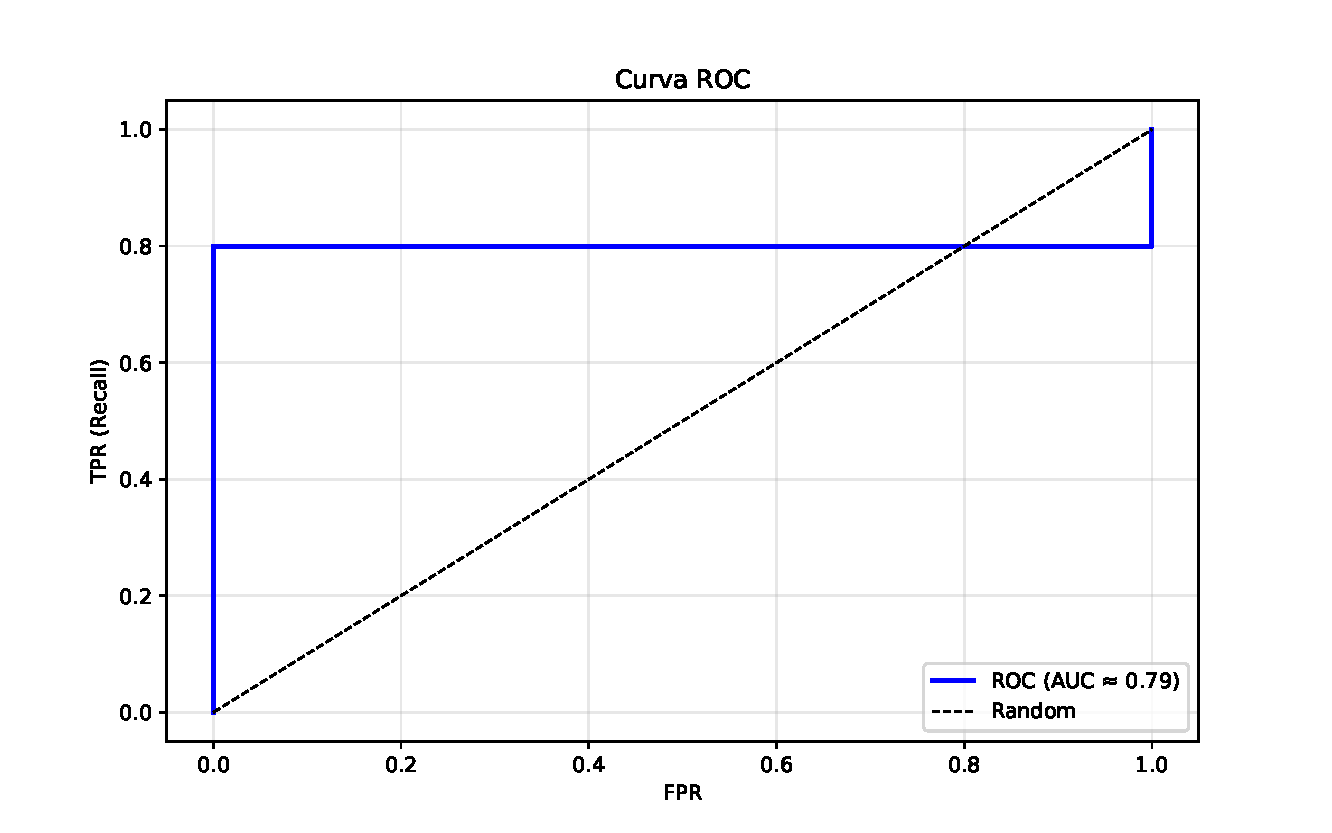
\includegraphics[width=0.85\textwidth]{LSTM/roc.pdf}
      \caption{Curva ROC y AUC del LSTM Autoencoder}
      \label{fig:roc_lstm}
\end{figure}

El resultado principal del proceso de validación se puede observar directamente en el siguiente gráfico, que muestra el momento exacto en que el modelo detecta una anomalía.

\begin{figure}[ht!]
      \centering
      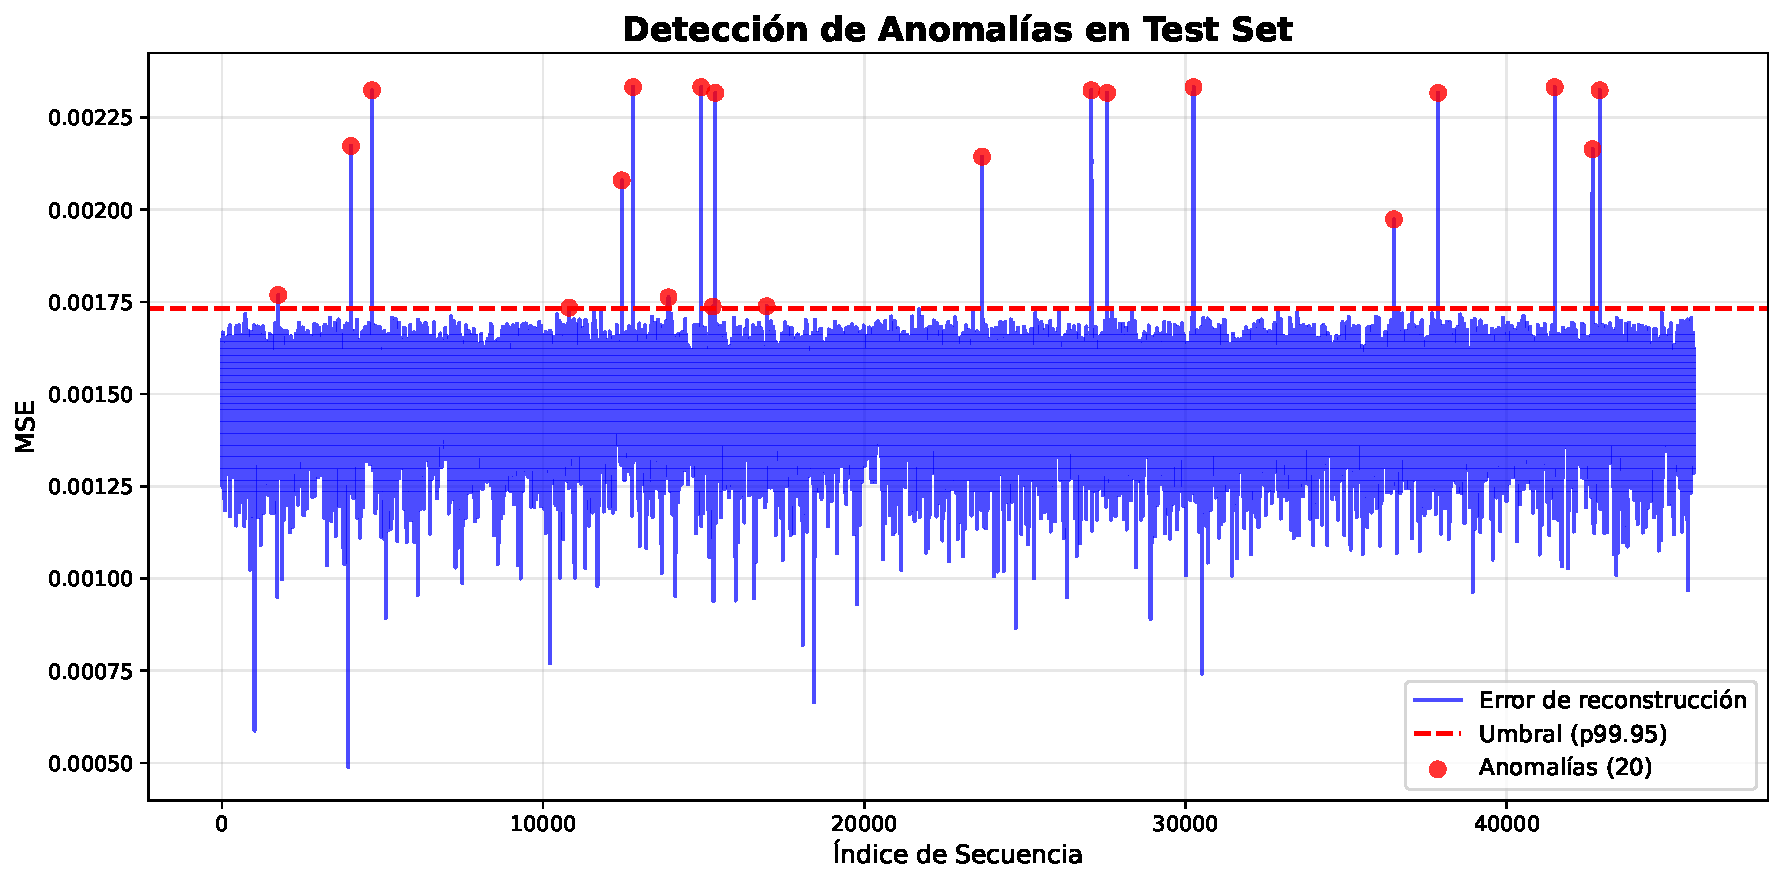
\includegraphics[width=0.85\textwidth]{LSTM/anomalias.pdf}
      \caption{Gráficas de MSE por secuencia para el LSTM Autoencoder.}
      \label{fig:mse_lstm}
\end{figure}

En la gráfica de la figura \ref{fig:mse_lstm}, se visualiza el error de reconstrucción para cada secuencia del conjunto de prueba. La línea discontinua roja representa el umbral de anomalía (MSE = 0.001646). Los puntos rojos marcan las 21 secuencias cuyo error superó este límite, siendo clasificadas correctamente como anomalías. Este gráfico confirma visualmente que el modelo es efectivo para asignar una puntuación de error mucho más alta a los eventos que se desvían del comportamiento normal aprendido.

Para analizar en detalle el rendimiento del modelo, no es suficiente con saber el número total de anomalías detectadas. Es fundamental comprender la naturaleza de sus aciertos y errores, y para ello se utiliza la matriz de confusión. Esta herramienta es una tabla que desglosa los resultados al comparar las predicciones del modelo con la realidad del conjunto de prueba, permitiéndonos visualizar cuatro escenarios clave:

\begin{itemize}
      \item Verdaderos Positivos (VP): Las anomalías que el modelo identificó correctamente.
      \item Verdaderos Negativos (VN): Los eventos normales que el modelo clasificó correctamente como normales.
      \item Falsos Positivos (FP): Eventos normales que el modelo etiquetó erróneamente como anomalías (las ``falsas alarmas'').
      \item Falsos Negativos (FN): Las anomalías reales que el modelo no fue capaz de detectar (los errores más críticos).
\end{itemize}

\begin{table}[ht!]
      \doublespacing
      \small
      \centering
      \begin{tabular}{ >{\centering\arraybackslash}p{3cm} >{\centering\arraybackslash}p{3cm} >{\centering\arraybackslash}p{3cm} }
            \hline
                          & \multicolumn{2}{c}{\textbf{Esperado}}              \\
            \hline
            \textbf{Real} & \textbf{P}                            & \textbf{N} \\
            \hline
            V             & 18                                    & 45814      \\
            F             & 3                                     & 6          \\
            \hline
      \end{tabular}
      \caption{Matriz de Confusión del LSTM Autoencoder}
      \label{tab:confusion_matrix_lstm}
\end{table}

VP (Verdaderos Positivos): 18

FP (Falsos Positivos): 3

FN (Falsos Negativos): 6

VN (Verdaderos Negativos): 45814

Estas cifras se traducen en las siguientes métricas de rendimiento:

\begin{itemize}
      \item  Exactitud (Accuracy): proporción de predicciones correctas respecto al total de casos evaluados.

            \begin{align}
                  Accuracy = \frac{TP+TN}{TP+TN+FP+FN}=\frac{(18+45814)}{(18+45814+3+6)}\approx 0.9998 \notag \\
                  \label{eq:accuracy}
            \end{align}
            \myequations{Accuracy para LSTM Autoencoder}


      \item Tasa de error: proporción de predicciones incorrectas respecto al total.

            \begin{align}
                  Error = \frac{FP+FN}{TP+TN+FP+FN}=\frac{(3+6)}{(18+45814+3+6)}\approx 0.0002 \notag \\
                  \label{eq:error}
            \end{align}
            \myequations{Tasa de Error para LSTM Autoencoder}

      \item Sensibilidad (Recall o Verdaderos Positivos): proporción de eventos de anomalos correctamente detectados.

            \begin{align}
                  Recall = \frac{TP}{TP+FN} \notag \\
                  \label{eq:recall}
            \end{align}
            \myequations{Recall para LSTM Autoencoder}

      \item Precisión: La proporción de casos realmente positivos entre todos los casos que el modelo predijo como positivos.

            \begin{align}
                  Precision = \frac{TP}{TP+FP}=\frac{18}{18+3}\approx 0.8571 \notag \\
                  \label{eq:precision}
            \end{align}
            \myequations{Precision para LSTM Autoencoder}

      \item Especificidad: proporción de eventos no críticos correctamente descartados.

            \begin{align}
                  Specificity = \frac{TN}{TN+FP}=\frac{45814}{45814+3}\approx 0.9999 \notag \\
                  \label{eq:specificity}
            \end{align}
            \myequations{Specificity para LSTM Autoencoder}

      \item F1 Score: media armónica entre la precisión y la sensibilidad, útil cuando es importante equilibrar ambas.

            \begin{align}
                  F1_{score} = 2 \cdot \frac{Precision \cdot Recall}{Precision + Recall} = 2 \cdot \frac{0.8571 * 0.75}{0.8571+0.75} \approx 0.8 \notag \\
                  \label{eq:f1score}
            \end{align}
            \myequations{F1 Score para LSTM Autoencoder}

\end{itemize}

El análisis de las métricas de rendimiento cuantifica el desempeño del modelo. La exactitud general es del 99.98\%, aunque este valor es menos indicativo en conjuntos de datos con clases desbalanceadas. Un análisis más específico muestra una Sensibilidad (Recall) del 75.0\%, lo que indica que el modelo identifica a tres de cada cuatro anomalías reales. A su vez, la Precisión es del 85.7\%, lo que significa que sus alertas positivas son correctas en esa proporción. La puntuación F1, como media armónica de ambas, se sitúa en 80.0\%, reflejando el balance entre la capacidad de detección y la fiabilidad de sus predicciones.

\uparagraph{Evaluacion del Isolation Forest}

Para la  evaluación del modelo Isolation Forest (IF), una técnica no supervisada que opera de manera fundamentalmente distinta al autoencoder. En lugar de medir un error de reconstrucción, este modelo asigna una ``puntuación de anomalía'' a cada evento basándose en qué tan fácil es aislarlo del resto de los datos. Los eventos que son más fáciles de separar (requieren menos divisiones en los árboles de decisión) se consideran más anómalos.

Funciona construyendo múltiples árboles de decisión (en este caso, 100) estos arboles se construyen al dividir aleatoriamente los datos en subconjuntos. Funciona bajo la premisa de que las anomalías son puntos de datos que se encuentran en regiones menos densas del espacio de características, por lo que son más fáciles de aislar. Cada evento recibe una puntuación basada en la profundidad promedio a la que aparece en los árboles; cuanto más cerca esté la puntuación de 1, más anómalo es el evento.

El proceso de evaluación se aplicó sobre el mismo conjunto de datos, compuesto por 100,809 registros, de los cuales 5,041 (5\%) son anomalías reales. A diferencia del LSTM Autoencoder, el umbral de decisión en el Isolation Forest no se calcula estadísticamente a posteriori, sino que se define a priori mediante el hiperparámetro contamination. Este valor se estableció en 0.05 (5\%), una práctica estándar para configurar este algoritmo. Cualquier evento cuya puntuación de anomalía superara el umbral derivado de esta configuración fue clasificado como anómalo.

\begin{figure}[ht!]
      \centering
      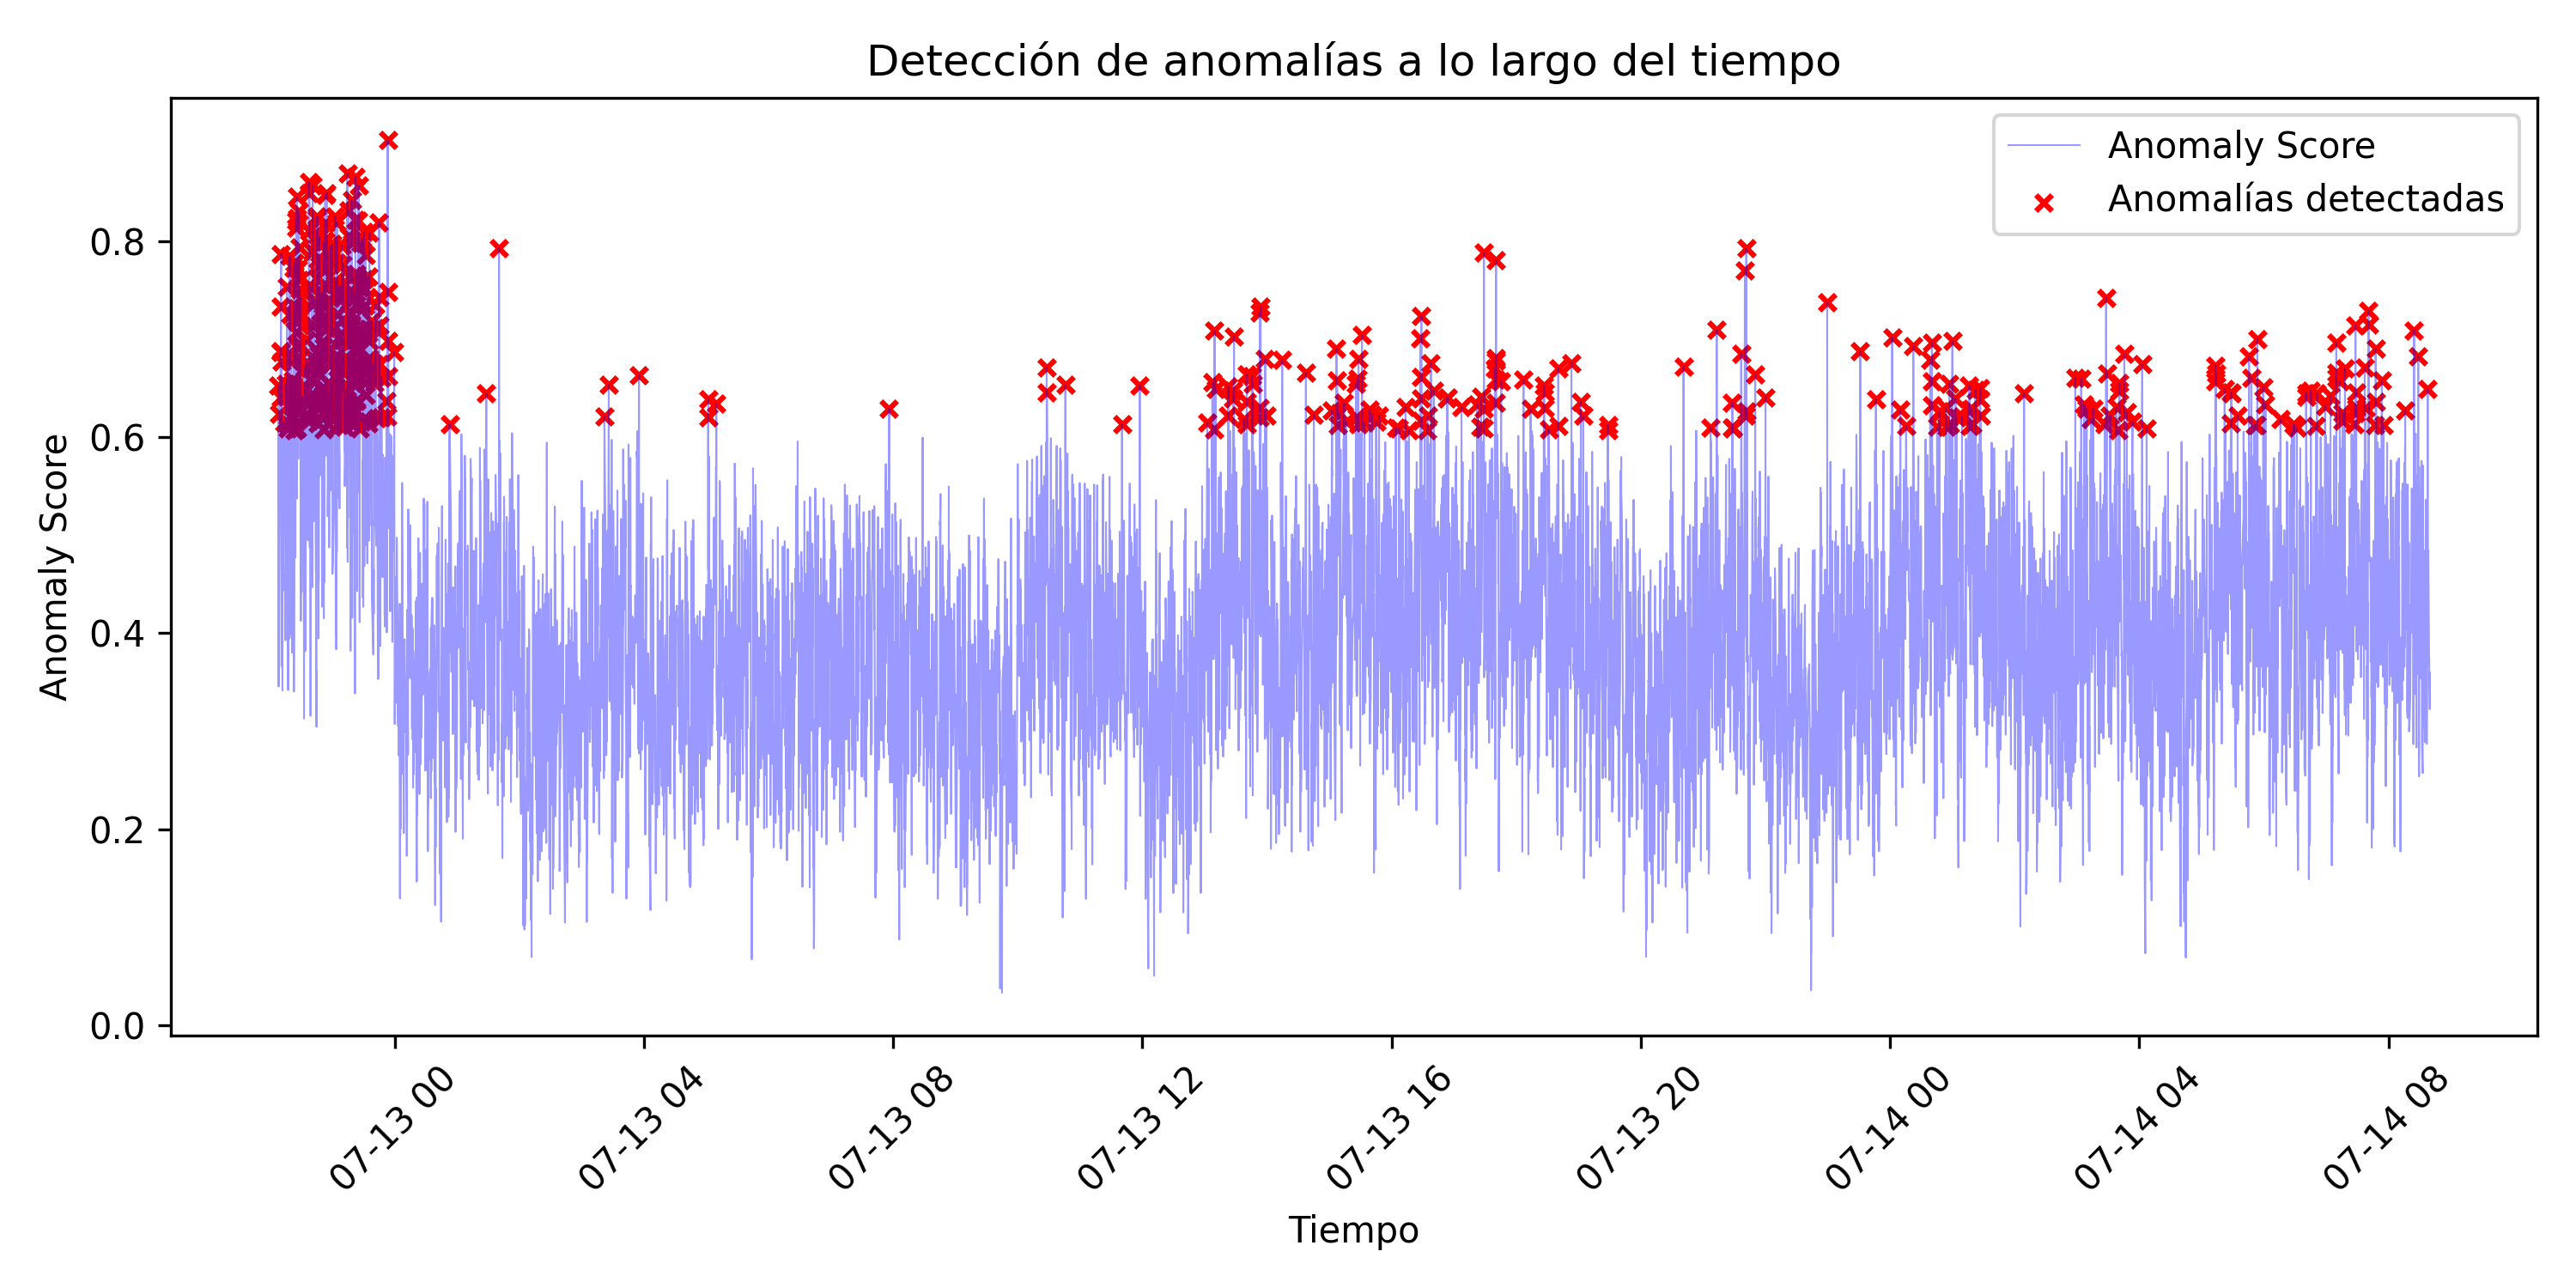
\includegraphics[width=0.85\textwidth]{IF/anomalias_tiempo.png}
      \caption{Gráficas de puntuación de anomalía por evento para el Isolation Forest.}
      \label{fig:anomalias_if}
\end{figure}

\begin{itemize}
      \item Análisis de la Detección

            El análisis de los resultados del Isolation Forest revela un rendimiento significativamente inferior al del LSTM Autoencoder. El modelo identificó un total de 5,041 eventos como anómalos. Sin embargo, un desglose más profundo a través de la matriz de confusión es necesario para entender la verdadera efectividad de estas detecciones.

            Para analizar en detalle el rendimiento del modelo, se utiliza la matriz de confusión. Esta herramienta desglosa los resultados al comparar las predicciones del modelo con la realidad del conjunto de prueba, permitiéndonos visualizar cuatro escenarios clave:

            \begin{table}[ht!]
                  \doublespacing
                  \small
                  \centering
                  \begin{tabular}{ >{\centering\arraybackslash}p{3cm} >{\centering\arraybackslash}p{3cm} >{\centering\arraybackslash}p{3cm} }
                        \hline
                                      & \multicolumn{2}{c}{\textbf{Esperado}}              \\
                        \hline
                        \textbf{Real} & \textbf{P}                            & \textbf{N} \\
                        \hline
                        V             & 2877                                  & 87737      \\
                        F             & 2164                                  & 8031       \\
                        \hline
                  \end{tabular}
                  \caption{Matriz de Confusión del Isolation Forest}
                  \label{tab:confusion_matrix_isolation_forest}
            \end{table}

            VP (Verdaderos Positivos): 2,877

            FP (Falsos Positivos): 2,164

            FN (Falsos Negativos): 8,031

            VN (Verdaderos Negativos): 87,737

            \begin{figure}[ht!]
                  \centering
                  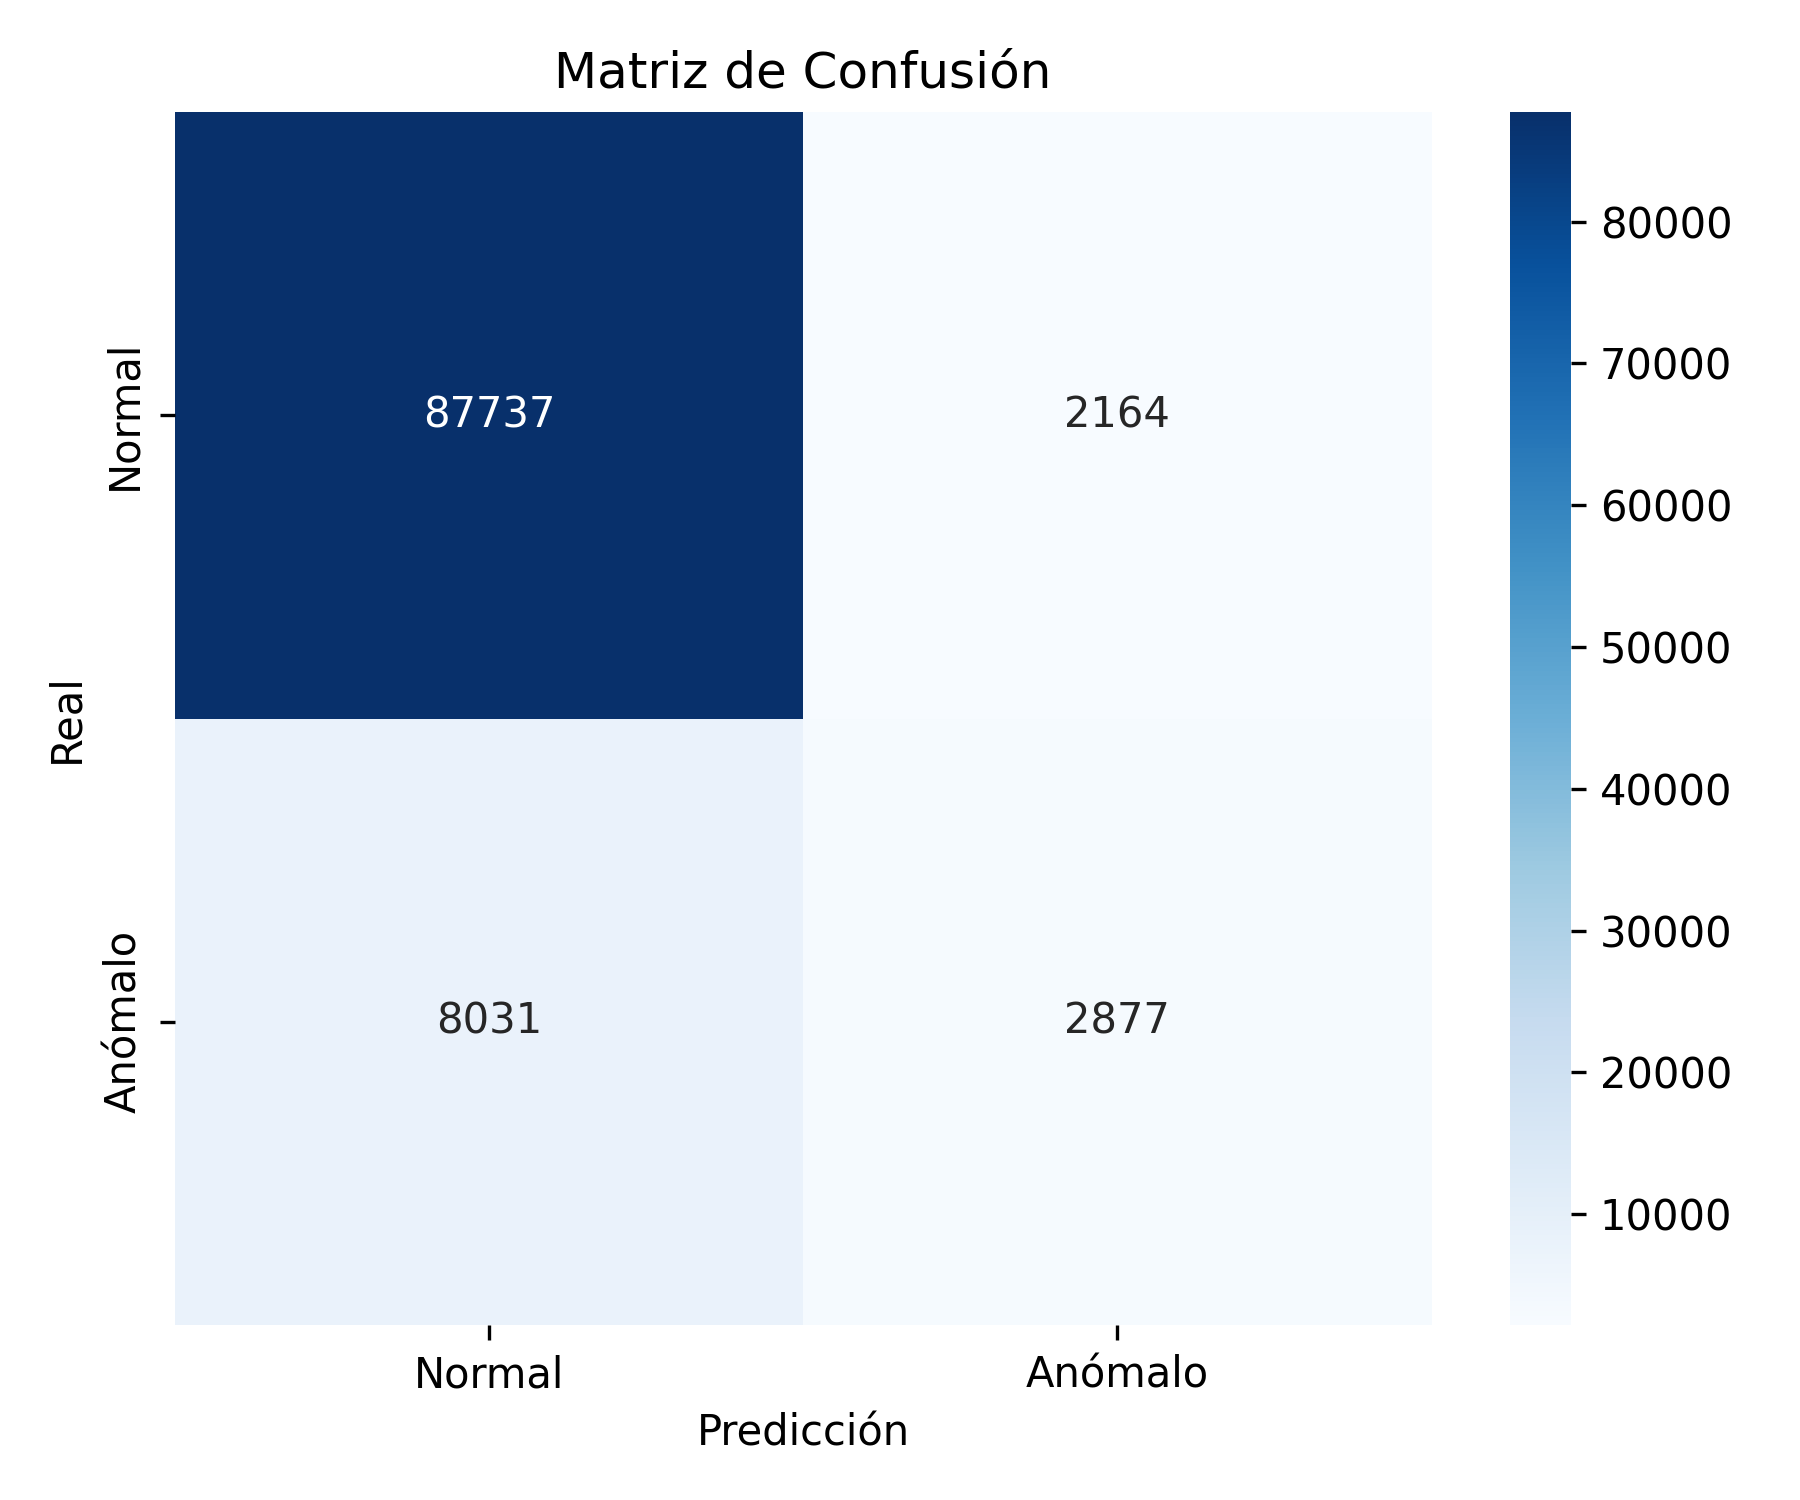
\includegraphics[width=0.65\textwidth]{IF/matriz_confusion.png}
                  \caption{Matriz de Confusión del Isolation Forest}
                  \label{fig:confusion_matrix_if}
            \end{figure}

      \item Métricas de Rendimiento

            \begin{align}
                  Accuracy = \frac{(2877+87737)}{(2877+87737+2164+8031)}\approx 0.8989 \notag \\
                  \label{eq:accuracy_if}
            \end{align}
            \myequations{Accuracy para Isolation Forest}


            \begin{align}
                  Error = \frac{(2164+8031)}{(2877+87737+2164+8031)}\approx 0.101 \notag \\
                  \label{eq:error_if}
            \end{align}
            \myequations{Tasa de Error para Isolation Forest}

            \begin{align}
                  Recall = \frac{2877}{2877+8031}\approx 0.2638 \notag \\
                  \label{eq:recall_if}
            \end{align}
            \myequations{Recall para Isolation Forest}

            \begin{align}
                  Precision = \frac{2877}{2877+2164}\approx 0.5707 \notag \\
                  \label{eq:precision_if}
            \end{align}
            \myequations{Precision para Isolation Forest}

            \begin{align}
                  Specificity = \frac{87737}{87737+2164}\approx 0.9759 \notag \\
                  \label{eq:specificity_if}
            \end{align}
            \myequations{Specificity para Isolation Forest}

            \begin{align}
                  F1_{score} = 2 \cdot \frac{Precision * Recall}{Precision+Recall} \notag \\
                  \label{eq:f1_if}
            \end{align}
            \myequations{F1 Score para Isolation Forest}

\end{itemize}

\begin{figure}[ht!]
      \centering
      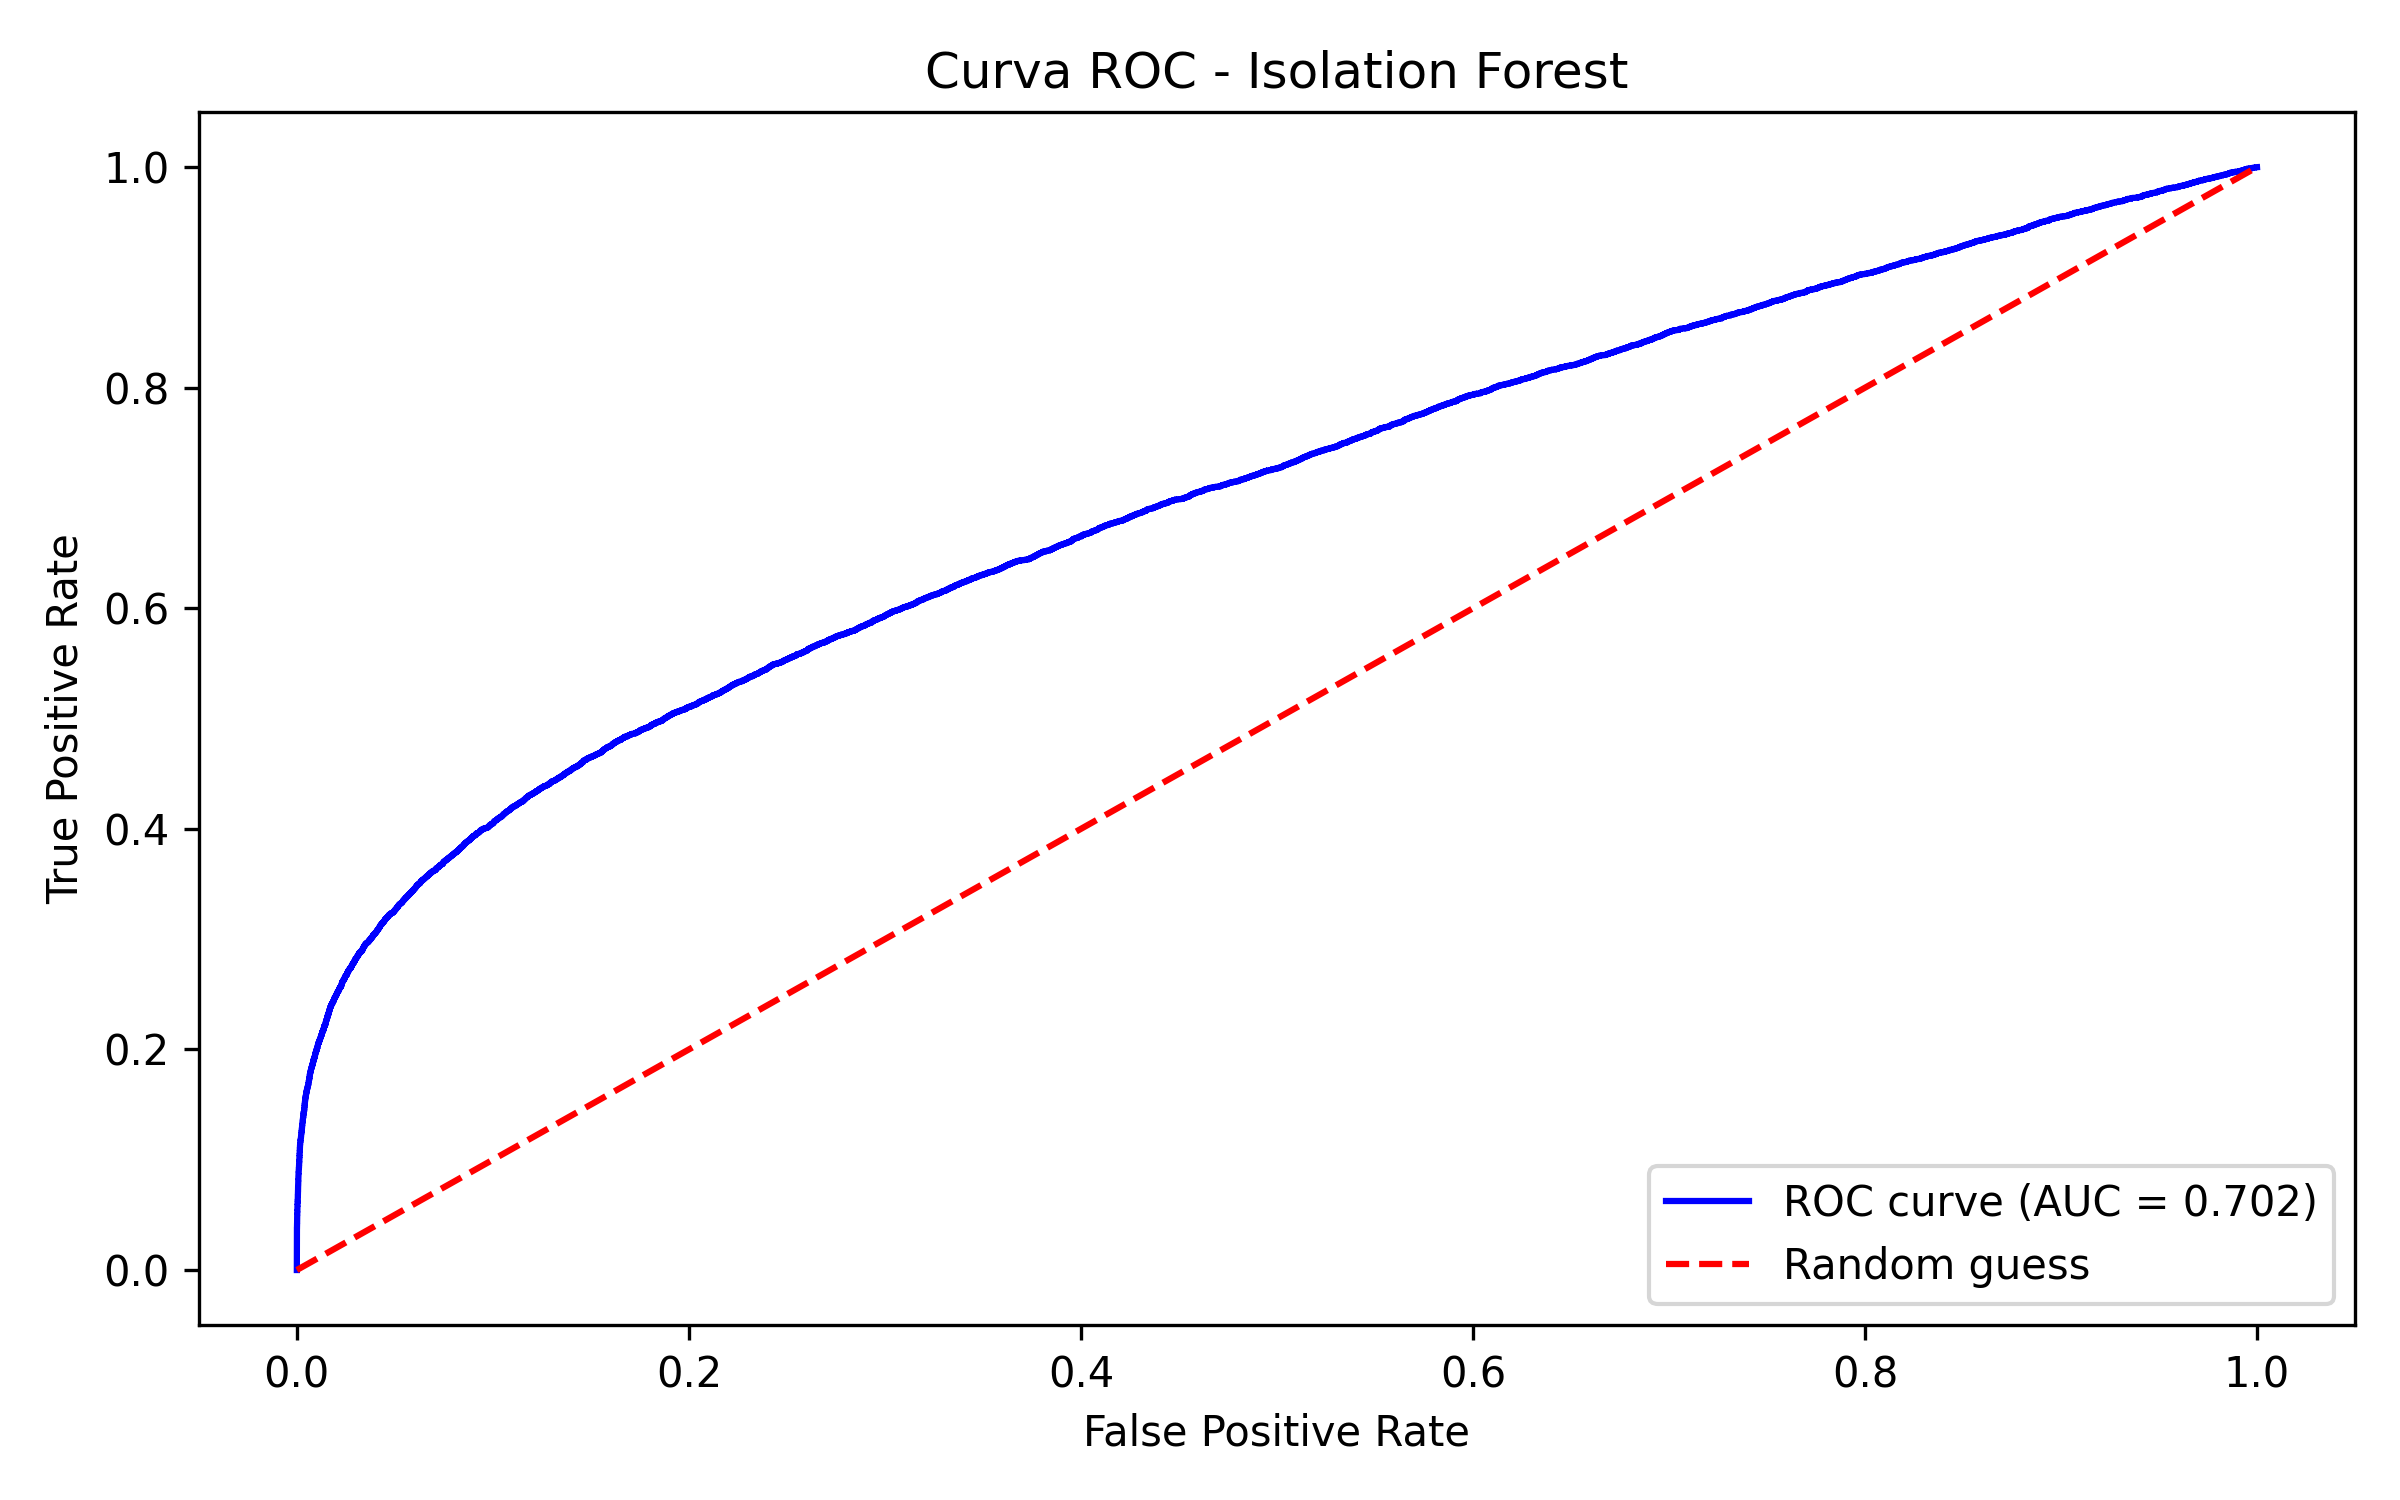
\includegraphics[width=0.85\textwidth]{IF/roc_auc.png}
      \caption{Curva ROC y AUC del Isolation Forest.}
      \label{fig:roc_if}
\end{figure}

El análisis de las métricas de rendimiento cuantifica el desempeño del modelo. La exactitud general del 89.9\% es un valor engañoso, inflado por la gran cantidad de eventos normales correctamente identificados. Las métricas más importantes revelan un rendimiento deficiente: una Sensibilidad (Recall) de solo el 26.4\%, lo que indica que el modelo no detectó a más de 3 de cada 4 anomalías reales. A su vez, la Precisión es del 57.1\%, lo que significa que casi la mitad de sus alertas son falsas alarmas. La puntuación F1 resultante, del 36.1\%, confirma que el modelo, en su configuración actual, carece de la capacidad necesaria para una detección fiable de anomalías en este contexto.

\usubsection{Validación del sistema de monitoreo acústico para generar alertas en casos de emergencia}